\section{Documentazione}
\subsection{Architettura del codice}
Il codice di laboratorio è diviso in tre sezioni principali: 
\begin{itemize}
	\item Implementazione delle strutture
	\item Implementazione dei test da effettuare
	\item Implementazione del \textit{plotter} dei grafici
\end{itemize}

La sezione relativa all'implementazione delle strutture dati, include tre file principali, ognuno dei quali contiene due classi: una per il nodo costituente e una per la struttura vera e propria. Il file \texttt{os\_ordered\_list.py} contiene l’implementazione della statistica d’ordine dinamica mediante lista ordinata, \texttt{os\_bst.py} quella basata sull’albero binario di ricerca e \texttt{os\_avl.py} l’implementazione tramite albero AVL.

Il file \texttt{test\_runner.py} contiene l'implementazione di tutti i test che devono essere effettuati e contiene inoltre, la funzione \text{main()}. 
Infine, il file \texttt{plot\_results.py} si occupa del salvataggio e lettura dei dati grezzi in formato \texttt{.csv}, oltre che alla generazione di ogni singolo grafico in formato \texttt{.pdf}.


\subsection{Implementazione delle strutture dati}
Per il diagramma UML completo delle classi fare riferimento alla Figura \ref{fig:uml_implementazioni}.

\subsubsection*{Lista Ordinata}
Per l'implementazione tramite lista ordinata si crea una lista doppiamente collegata. Di fatto ogni \texttt{OrderedListNode} avrà tre attributi fondamentali: la chiave \texttt{key}, il puntatore al nodo successivo \texttt{next} e il puntatore al nodo precedente \texttt{prev}. Il nodo in testa alla lista avrà \texttt{prev}$= \text{null}$, mentre l'ultimo nodo della coda avrà \texttt{next}$= \text{null}$.

Di sotto si riporta la spiegazione dei metodi della lista ordinata.
\begin{itemize}
	\item \texttt{insert(key)}: inserisce in maniera ordinata un nuovo elemento di chiave \texttt{key} nella lista.
	\item \texttt{delete(key)}: rimuove il primo elemento di chiave \texttt{key} dalla lista. Se l'elemento non è presente scorre tutta la lista. In seguito all'eliminazione vengono aggiustati i puntatori dei nodi adiacenti a quello eliminato in maniera corretta.
	\item \texttt{print(key)}: scorre la lista e stampa ogni elemento in ordine.
	\item \texttt{select(i)}: restituisce la chiave dell'i-esimo nodo all'interno della lista
	\item \texttt{rank(key)}: restituisce la posizione a partire dalla testa della lista (rango) del nodo di chiave \texttt{key}.
\end{itemize} 

\subsubsection*{Albero Binario di Ricerca}
Il singolo nodo dell’ABR, \texttt{BSTNode}, è stato implementato mediante i seguenti attributi: la chiave \texttt{key}, il puntatore al figlio destro \texttt{right}, il puntatore al figlio sinistro \texttt{left} e il puntatore al nodo genitore \texttt{parent}. Il nodo radice, \texttt{root}, è l’unico nodo per cui il puntatore \texttt{parent} risulta nullo.


Per l'ABR sono stati implementati i seguenti metodi:
\begin{itemize}
	\item \texttt{insert(key)}: inserisce l'emento di chiave $key$ all'interno dell'albero nella posizione corretta.
	\item \texttt{delete(key)}: rimuove l'elemento di chiave $key$ dall'albero effettuando in seguito una ristrutturazione per ricollegare i nodi in maniera corretta. Fa uso del metodo \texttt{successor()}.
	\item \texttt{print(key)}: metodo implementato per avere la stessa interfaccia fra le tre implementazioni. Chiama al suo interno il metodo \texttt{inorder\_tree\_walk()}.
	\item \sloppy \texttt{select(i)}: esplora l'albero e restituisce il nodo in posizione i-esima rispetto ad un \texttt{inorder\_tree\_walk()}.
	\item \texttt{rank(key)}: esplora l'albero e restituisce la posizione rispetto ad un \texttt{inorder\_tree\_walk()} del nodo di chiave \texttt{key}.
	\item \texttt{min(node)}: restituisce il nodo con la chiave più piccola. Per costruzione è il successore più a sinistra.
	\item \texttt{max(node)}: restituisce il nodo con la chiave più grande. Per costruzione è il successore più a destra.
	\item \texttt{find(node, key)}: cerca il nodo con la chiave \texttt{key}. Se non viene trovato restituisce \textit{None}.
	\item \texttt{successor(node)}: restituisce il successore del nodo \textit{node}. Fa uso del metodo \texttt{min()}.
	\item \texttt{inorder\_tree\_walk(node)}: effettua un attraversamento ordinato dell'albero. Stampando gli elementi dal più piccolo al più grande.
	\item \texttt{size(node)}: Conta quanti nodi si trovano nei due sottoalberi destro e sinistro di \texttt{node}, compreso \texttt{node} stesso.
\end{itemize}

\subsubsection*{Albero AVL}
Il singolo nodo dell'Albero AVL, \texttt{AVLNode} è stato implementato con $5$ attributi: la chiave \texttt{key}, il puntatore al figlio destro \texttt{right}, il puntatore al figlio sinistro \texttt{left}, l'attributo \texttt{height} che tiene traccia del numero di archi nel percorso più lungo dal nodo alla foglia e, infine, l'attributo \texttt{size} che tiene traccia del numero totale di nodi nei sottoalberi destro e sinistro compreso il nodo radice. Quest'ultimo attributo è l'analogo del metodo \texttt{size(node)} dell'ABR che viene aggiornato solo quando modifico la struttura dell'albero, risparmiando così risorse computazionali.

Di sotto in dettaglio i metodi della classe:
\begin{itemize}
	\item \texttt{insert(key)}: inserisce l'emento di chiave \texttt{key} all'interno dell'albero nella posizione corretta. Effettua una rotazione appropriata per mantenere il \texttt{balance\_factor}$\in [-1, 0, 1]$, utilizzando i metodi \texttt{right\_rotate()} e \texttt{left\_rotate()}.
	\item \texttt{delete(key)}: rimuove l'elemento di chiave \textit{key} dall'albero effettuando in seguito una ristrutturazione tramite rotazioni per bilanciare i nodi in maniera corretta. Fa uso del metodo \texttt{successor()}.
	\item \texttt{print(key)}: metodo implementato per avere la stessa interfaccia fra le tre implementazioni. L'unica cosa che fa è chiamare il metodo \texttt{inorder\_tree\_walk()}.
	\item \sloppy \texttt{select(i)}: esplora l'albero e restituisce il nodo in posizione i-esima rispetto ad un \texttt{inorder\_tree\_walk()}.
	\item \texttt{rank(key)}: esplora l'albero e restituisce la posizione rispetto ad un \texttt{inorder\_tree\_walk()} del nodo di chiave \texttt{key}.
	\item \texttt{get\_height(node)}: restituisce l'altezza del nodo \texttt{node}.
	\item \texttt{get\_size(node)}: restituisce la dimensione del nodo \texttt{node}.
	\item \texttt{get\_balance(node)}: restituisce il fattore di bilanciamento del nodo \texttt{node}.
	\item \texttt{update(node)}: metodo di supporto. Ricalcola e aggiorna gli attributi \texttt{height} e \texttt{size} del nodo \texttt{node}.
	\item \texttt{right\_rotate(node)}: effettua una rotazione a destra dell'albero.
	\item \texttt{left\_rotate(node)}: effettua una rotazione a sinistra dell'albero.
	\item \texttt{min(node)}: restituisce il nodo con la chiave più piccola. Per costruzione è il successore più a sinistra.
	\item \texttt{max(node)}: restituisce il nodo con la chiave più grande. Per costruzione è il successore più a destra.
	\item \texttt{successor(node)}: restituisce il successore del nodo \texttt{node}. Fa uso del metodo \texttt{min()}.
	\item \texttt{inorder\_tree\_walk(node)}: effettua un attraversamento ordinato dell'albero stampando gli elementi dal più piccolo al più grande.
\end{itemize}

\begin{figure}[H]
	\centering
	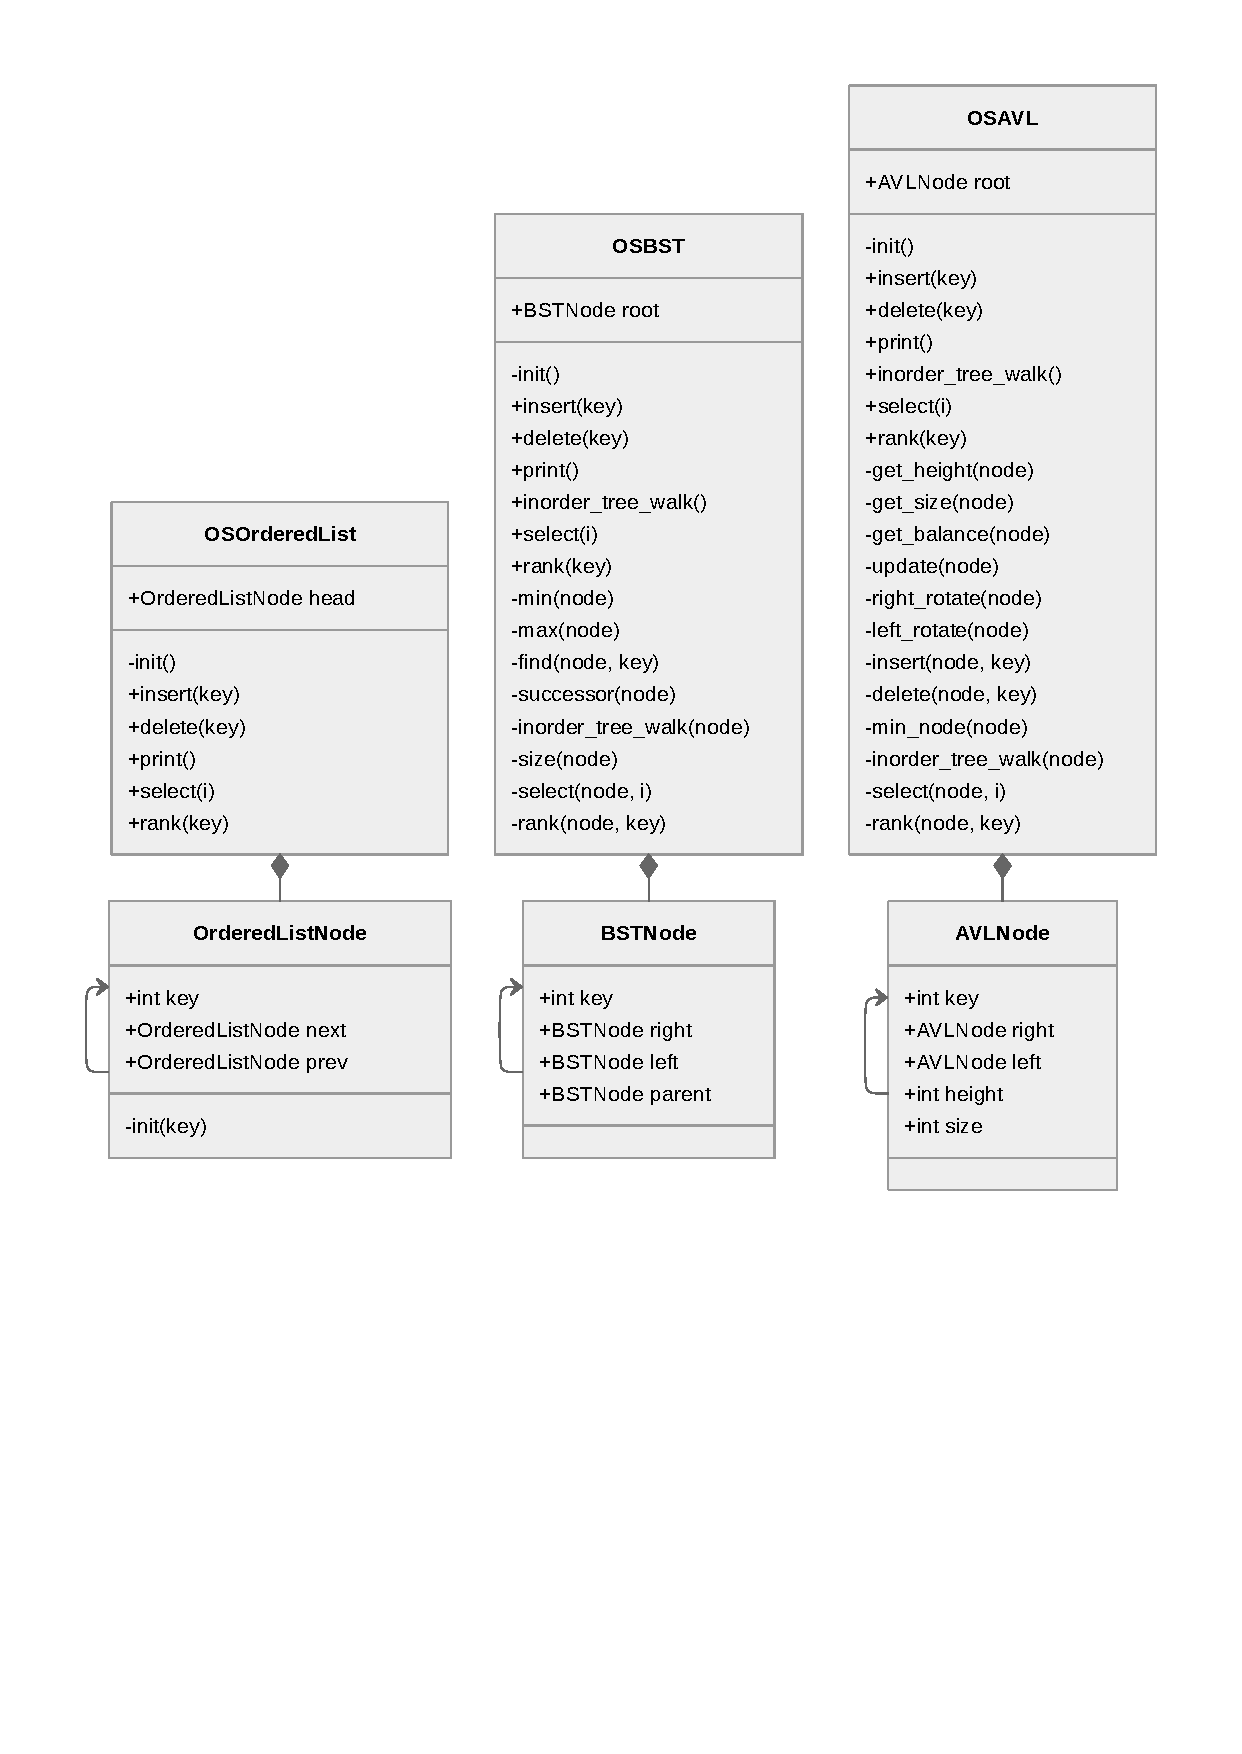
\includegraphics[width=1\textwidth]{figures/uml_implementazione_strutture.pdf}
	\caption{Diagramma UML delle tre implementazioni}
	\label{fig:uml_implementazioni}
\end{figure}

\subsection{Implementazione degli esperimenti}
Gli esperimenti sono stati condotti confrontando le tre strutture dati implementate, \texttt{OSOrderedList}, \texttt{OSBST} e \texttt{OSAVL}, su $5$ condizioni distinte, al variare della dimensione dell'input. In tutti i test il numero massimo di elementi inseriti è fissato a \texttt{size}$= 5000$, ad eccezione del test di \textit{inserimento ordinato} il cui limite è fissato ad un terzo di quello degli altri ovvero \texttt{size}$= \lfloor\frac{5000}{3}\rfloor = 1666$ elementi. Ogni test procede eseguendo il controllo su insiemi di elementi che crescono di un passo \texttt{step}$= 50$, fino a che non si raggiunge la quantità \texttt{size}. Per ognuno di questi passi il test viene eseguito \texttt{repetitions}=$10$ volte. Il risultato di ogni ripetizione viene salvato in una lista ed in fine viene preso il valore mediano al fine di limitare le fluttuazioni date dagli inserimenti casuali che potrebbero generare delle sequenze favorevoli o sfavorevoli. Il valore sarà il dato salvato nel file \texttt{.csv}. 

\begin{itemize}
	\item \texttt{test\_casual\_input}: misura il tempo di inserimento di sequenze di valori casuali distinti, estratti senza rimpiazzo dall'intervallo $[1,\, 10^7]$.
	\item \texttt{test\_ordered\_input}: misura il tempo di inserimento di sequenze ordinate in senso crescente $0, 1, 2, \dots$, caso particolarmente sfavorevole per il BST non bilanciato poiché degenera in una lista.
	\item \texttt{test\_casual\_deletion}: le strutture vengono prima popolate con una sequenza casuale di $x$ elementi, dopodiché si elimina un sottoinsieme casuale di $\lfloor x/2 \rfloor$ elementi presenti nella struttura.
	\item \texttt{test\_casual\_ranking}: analogamente al test precedente, le strutture vengono pre-popolate con $x$ elementi casuali; si misura poi il tempo necessario a eseguire l'operazione \texttt{rank} su $\lfloor x/2 \rfloor$ chiavi scelte casualmente tra quelle inserite.
	\item \texttt{test\_casual\_selection}: le strutture vengono pre-popolate con $x$ elementi casuali; si misura il tempo per eseguire l'operazione \texttt{select} su $\lfloor x/2 \rfloor$ indici interi scelti uniformemente a caso nell'intervallo $[1,\, x]$.
\end{itemize}

\subsubsection*{Creazione dei grafici}
Nel file \texttt{plot\_results.py} sono state implementate alcune funzioni il cui scopo è scrivere, leggere e rappresentare i risultati sperimentali. 
\begin{itemize}
	\item \texttt{conv\_pascal\_case(file\_name)}: si occupa di modificare il nome del file cambiandolo da \textit{snake\_case} a \textit{Pascal Case} in modo che possa essere stampato assieme al grafico come didascalia.
	\item \texttt{save\_csv(file\_name, rows)}: si occupa di salvare i dati in un file \texttt{.csv} il cui nome corrisponde al tipo di test effettuato.
	\item \texttt{read\_csv(file\_name)}: si occupa di prendere il file \texttt{.csv} corretto e restituire una lista coi dati d'interesse che devono essere messi in grafico dalla funzione \texttt{plot()}.
	\item \texttt{plot(file\_name)}: si occupa di creare i grafici dei dati e salvare le figure generate in formato \texttt{.pdf}.
\end{itemize}

\newpage